165. \begin{figure}[ht!]
\center{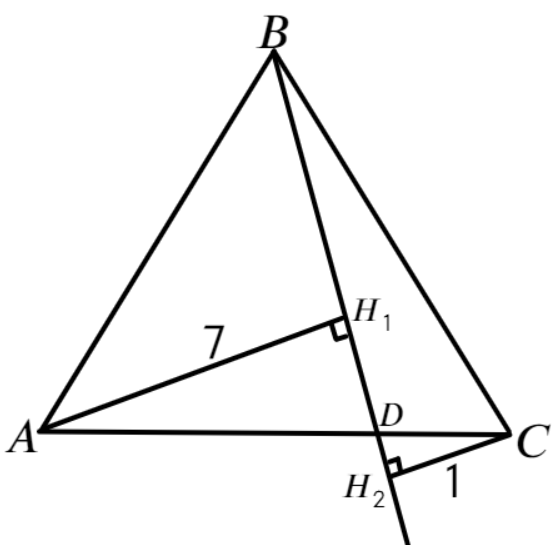
\includegraphics[scale=0.35]{g8-165.png}}
\end{figure}\\
Треугольники $AH_1D$ и $CH_2D$ подобны по двум углам (прямым и вертикальным), значит $\cfrac{AD}{DC}=\cfrac{AH_1}{CH_2}=7.$ Если сторона правильного треугольника равна $a,$ то $AD=\cfrac{7}{8}a,\ DC=\cfrac{1}{8}a.$ Воспользовашись теоремой Пифагора для треугольников $CDH_2,\ ABH_1,\ ADH_1$ и $BCH_2,$ получим $DH_2=\sqrt{\cfrac{a^2}{64}-1},\ DH_1=\sqrt{\cfrac{49a^2}{64}-49},\ BH_1=\sqrt{a^2-49},\ BH_2=\sqrt{a^2-1}.$ Тогда
$\sqrt{a^2-1}=\cfrac{\sqrt{a^2-64}}{8}+\cfrac{7\sqrt{a^2-64}}{8}+\sqrt{a^2-49},\
\sqrt{a^2-1}=\sqrt{a^2-64}+\sqrt{a^2-49}.$ Сделаем замену $x=a^2-64,$ тогда $\sqrt{x+63}=\sqrt{x}+\sqrt{x+15}\Leftrightarrow x+63=x+x+15+2\sqrt{x(x+15)}\Leftrightarrow 2\sqrt{x(x+15)}=48-x$\\$ \Leftrightarrow \begin{cases} 4x^2+60x=2304-96x+x^2,\\ x\leqslant 46.\end{cases}
\Leftrightarrow \begin{cases} 3x^2+156x-2304=0,\\ x\leqslant 46.\end{cases}
\Leftrightarrow \begin{cases} x^2+52x-768=0,\\ x\leqslant 46.\end{cases}\Leftrightarrow x=12$ или $x=-64.$
Тогда $a=\sqrt{x+64}=\sqrt{96}=2\sqrt{19},$ во втором случае $a=0,$ что невозможно.
ewpage
oindent
